\subsection{Data Types}
    Data types represent different numerical formats within a process control system. The below list defines the basic data types used within a process control system.
    
    \subsubsection{BIT}
        Bits are binary values that can be either of two values, 1 or 0. Digital \acrshort{io} used within the lolly machine are all triggered by binary variables as the only two options are on (1) or off (0). 
    
    \subsubsection{BYTE}
        1 Byte is 8 bits. A BYTE can be represented in binary or by 2 hexadecimal characters.
    
    \subsubsection{WORD}
        1 Word is 2 Bytes which is 16 bits as illustrated in Figure \ref{fig:word}. A WORD can be represented in binary or by 4 hexadecimal characters.
        \begin{figure}[H]
            \centering
            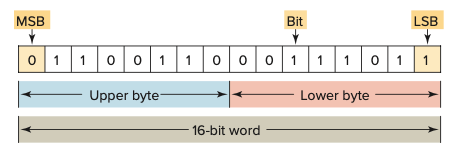
\includegraphics[width = 0.5\textwidth]{2_images/word.png}
            \caption{A 16 bit word \cite{petruzella2017programmable}.}
            \label{fig:word}
        \end{figure}           
        
    
    \subsubsection{\acrfull{dword}}
        1 Double Word is 2 Words which is 32 bits. A \acrshort{dword} can be represented in binary or by 8 hexadecimal characters.
 \newpage   
    \subsubsection{\acrfull{int}}
        An \acrshort{int} is a 16 bit number which can be either signed or unsigned. A signed \acrshort{int} ranges from -32,768 to 32,767 while an unsigned \acrshort{int} ranges from 0 to 65,535\cite{dataTypesSiemens}. Figure \ref{fig:int} illustrates how an 8 bit unsigned integer is represented in twos compliment - the same technique is applicable to 16 and 32 bit numbers.
        \begin{figure}[H]
            \centering
            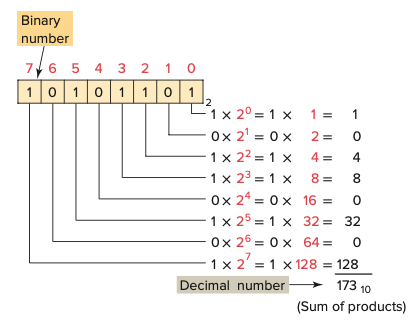
\includegraphics[width = 0.4\textwidth]{2_images/int.png}
            \caption{An 8 bit integer \cite{petruzella2017programmable}.}
            \label{fig:int}
        \end{figure}         
        
    
    \subsubsection{\acrfull{dint}}
        A \acrshort{dint} is a 32 bit number which can be either signed or unsigned. A signed \acrshort{dint} ranges from -2,147,483,648 to 2,147,483,647 while an unsigned is 0 to 4,294,967,295 \cite{dataTypesSiemens}. 
        
        \subsubsection{\acrfull{real}}
        A \acrshort{real} is a 32 bit number that represents real or floating point number. A \acrshort{real} can range from +/-1.18 x 10 $^{-38}$ to +/-3.40 x 10 $^{38}$ \cite{dataTypesSiemens}. A \acrshort{real} has three separate parts these are\cite{petruzella2017programmable}:
        
        \begin{description}
            \item\textbf{Sign}: 1 bit that defines the sign of the number.
            \item\textbf{Mantissa}: 23 bits, representing the significant figures.
            \item\textbf{Exponent}: 8 bits, representing the positive or negative power that the mantissa is raised.
        \end{description}
        
        \begin{figure}[H]
            \centering
            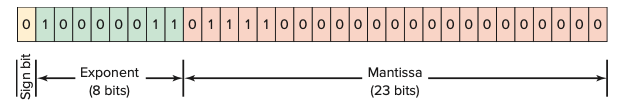
\includegraphics[width = 0.7\textwidth]{2_images/real.png}
            \caption{A \acrfull{real} word \cite{petruzella2017programmable}.}
            \label{fig:real}
        \end{figure}  
\newpage
\subsection{Serial Communication}
    Communication between devices can be achieved through serial communication. The base premise of serial communication is that data is sent one bit at a time \cite{frenzel2015handbook}. Bits are transmitted through a copper cable where differing voltage levels are inferred as either a 0 or 1\cite{frenzel2015handbook}. To understand serial communications properly there are a few terms that should be understood.
    \begin{description}
        \item\textbf{Baud Rate:} The number of bits that are transmitted or received per 1 second.
        \item\textbf{Telegram:} The complete set of data per transmission, comprising of 'n' number of bits which is dependent on the protocol.
        \item\textbf{\acrshort{lsb}:} The least significant bit in telegram.
        \item\textbf{\acrshort{msb}:} The most significant bit in telegram.
        \item\textbf{Parity Bit:} An optional check bit which is typically located at the \acrshort{lsb}. Parity can be either odd or even. Even parity means that there are an even number of 1s in a string while odd parity is an odd number of 1s in a string.
        \item\textbf{Start/ Stop-Bit:} A start bit defines the beginning of a telegram while a stop bit defines the end.
        \item\textbf{Half/ Full-Duplex} Half duplex means that data can be sent or received at any one point in time - data cannot be send and received synchronously. Full Duplex means that data can be sent and received at the same time.
    \end{description}
    Varying standards define different methods of serial communication. The lolly machine has two different serial communications standards. 
    
    % could also include spi and i2c but we will see. . . 
    \newpage
    \subsubsection{RS-232}
        RS-232 is a full-duplex, multi-wire, point-to-point system where a computer or terminal device, \acrfull{dte} communicates with various types of of \acrfull{dce}\cite{frenzel2015handbook}. 
        \begin{description}
            \item\textbf{Logic Levels:}
            \item0: +3V to +25V, Typically +5 to +12V
            \item1: -3V to -25V, Typically -5 to -12
        \end{description}
        
        An RS-232 port on the \acrshort{plc} provides a method of connection from the engineering workstation. The initial setup of the \acrshort{plc} must be made through this port as there are is no default \acrshort{ip} address.
        Figure \ref{fig:rs232Trans} illustrates an RS-232 data transmission.
        
        \begin{figure}[H]
            \centering
            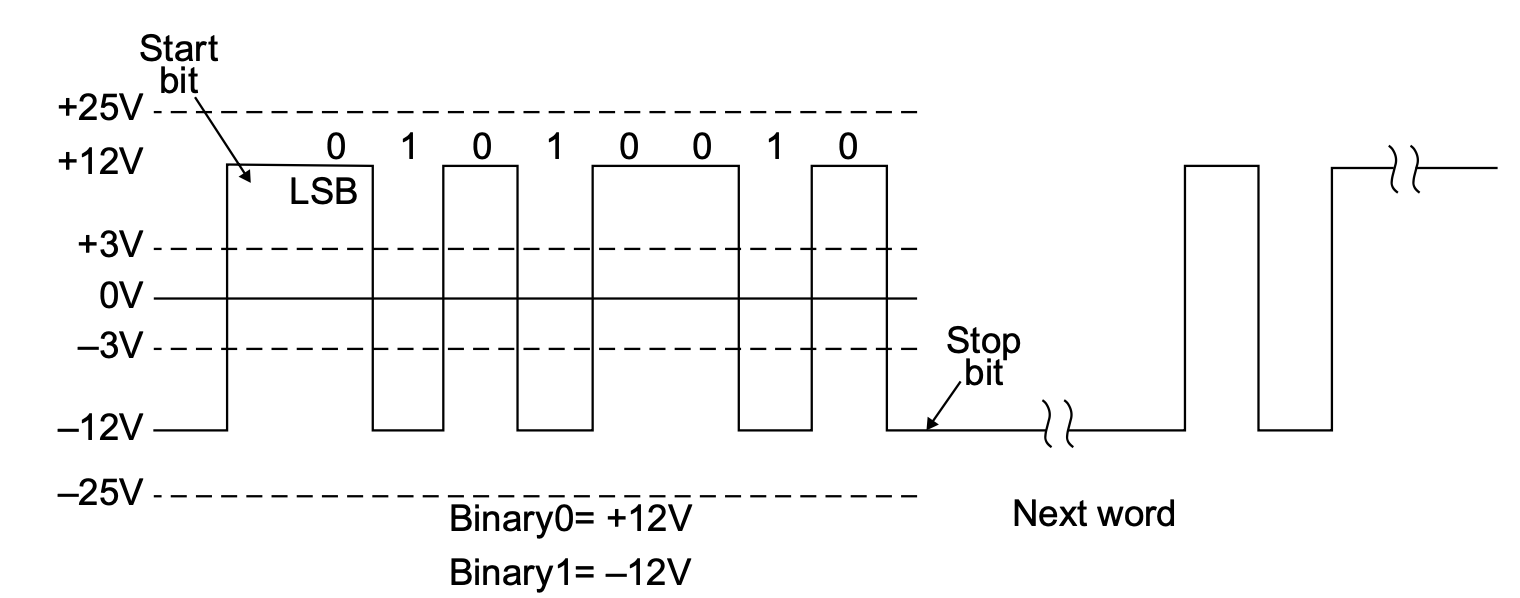
\includegraphics[width = 0.7\textwidth]{2_images/rs232Trans.png}
            \caption{A RS-232 data transmission~\cite{frenzel2015handbook}.}
            \label{fig:rs232Trans}
        \end{figure} 
    \newpage    
    \subsubsection{RS-485}
       RS-485 is a half-duplex, multi drop communication standard capable of supporting up to 32 nodes, each having transmitters and receivers. Voltages are taken across a differential pair which reduces the affect of noise on the system.  Data can be from 5 to 8 bits in length. Figure \ref{fig:rs485Nodes} shows a standard network configuration which includes two 120 ohm resistors which are used to combat reflections.

        \begin{figure}[H]
            \centering
            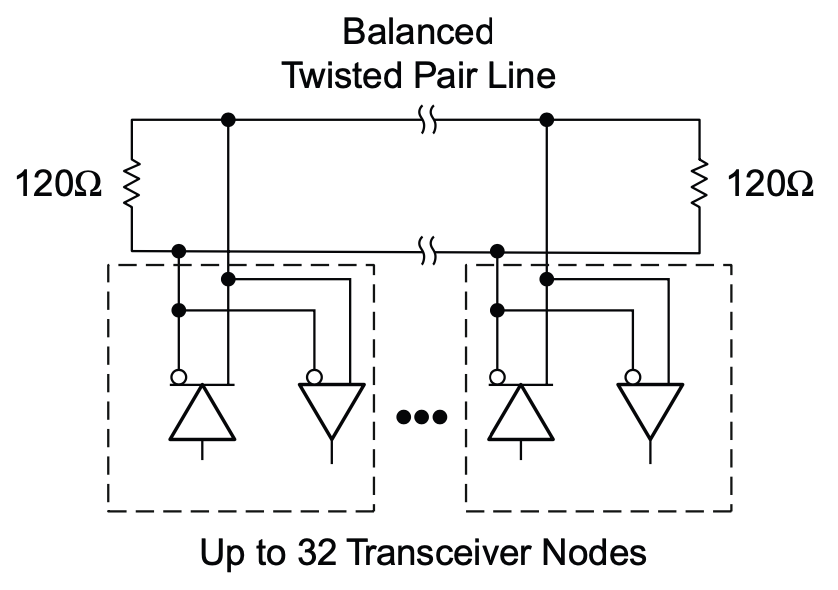
\includegraphics[width = 0.5\textwidth]{2_images/rs485Nodes.png}
            \caption{Configuration of a RS-485 network~\cite{frenzel2015handbook}.}
            \label{fig:rs485Nodes}
        \end{figure}        
       
       
        \begin{description}
            \item\textbf{Logic Levels:}
            \item0: +1.5V to +6V
            \item1: -1.5V to -6V
        \end{description}       
       
        An RS-485 port on the \acrshort{plc} is utilised to communicate with the Arduino through a RS-485 to \acrshort{ttl} converter.
     
\newpage    
\subsection{Ethernet}
    Ethernet, also known as IEEE 802.3, is a commonly used communication standard that governs the Physical and Data-Link Link layers (in relation to the \acrshort{osi}\footnote{The \acrshort{osi} model provides a framework that describes how applications can communicate over a wired \acrshort{lan}\cite{scott2021networking}.} model shown in Figure \ref{fig:osi}) of a wired \acrshort{lan}\cite{scott2021networking}. A wired \acrfull{lan} is a group of network devices that are connected on a local Ethernet network.  
    
        \begin{figure}[H]
            \centering
            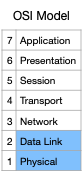
\includegraphics[width = 0.1\textwidth]{2_images/osi.png}
            \caption{The \acrshort{osi} model\cite{scott2021networking}.}
            \label{fig:osi}
        \end{figure} 
    
    An Ethernet network is established through physical cabling. Cabling can be coaxial, twisted copper pairs of fibre optic \cite{scott2021networking}.
    
    All devices on the lolly machine support Ethernet, subsequently all devices are on the same \acrshort{lan}.
    
    Each Ethernet device has a unique address which is called an \acrshort{ip} address. An \acrshort{ip} address is a four-octet, eight-bit address\cite{scott2021networking}.  
    
            \begin{figure}[H]
            \centering
            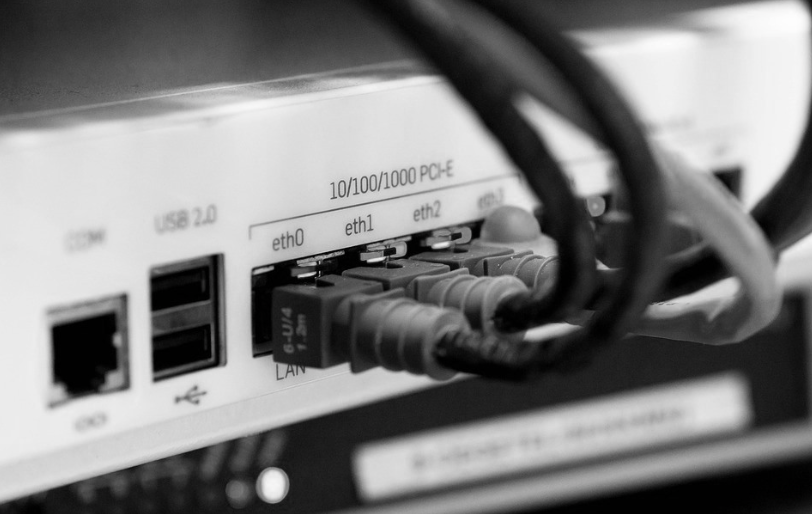
\includegraphics[width = 0.6\textwidth]{2_images/ethernetCables.png}
            \caption{Ethernet cables plugged into a network switch\cite{scott2021networking}.}
            \label{fig:ethenetCables}
        \end{figure} 
\newpage    
\subsection{Modbus}
    Modbus is an open-source \footnote{Open-source means that the developers have made the protocol available to the public. This allows third parties to use the protocol in their own products.} communication protocol that was produced by Modicon \cite{frenzel2015handbook}. Modbus was originally used exclusively in serial networks (RS-232 and RS-485) but has now expanded to TCP/IP which runs over an Ethernet network\cite{frenzel2015handbook}. 
    
    There are two main types of devices in a Modbus network, the Master and Slave\cite{frenzel2015handbook}. The Master can request data from a slave but not vice versa. A Master cannot request data from another master and a slave cannot request data another slave. Some devices like \acrshort{plc}s can be Mater/Slaves allowing inter \acrshort{plc} communication and tiered hierarchy of control. E.g., the \acrshort{hmi} on the lolly machine controls the \acrshort{plc} and the \acrshort{plc} controls the remote \acrshort{io}. Modbus on an Ethernet network operates on the same principles as those describe above however, the terminology is slightly different. A Master device is referred to as a Client while a Slave device is referred to as a Server. A way to remember this is that a server "serves" the client.
    
    In a Modbus network, data is communicated between devices in single bits or in WORDs (2 BYTES). 
    The Modbus protocol has four different address types, these are as follows:
    
    \begin{description}
        \item\textbf{Coil:} 1 bit - Read/ Write Access
        \item\textbf{Discrete Input:} 1 bit - Read Only Access
        \item\textbf{Input Register:} 16 bit WORD - Read Only Access
        \item\textbf{Holding Register:} 16 bit WORD - Read/ Write Access
    \end{description}
    
    When the Master/ Client device requests data from the Slave/ Server, it does so with a function code. The function code lets the Slave/ Server know how to respond to the request. The below list shows what each code corresponds to. 
    
    \begin{center}
        \begin{tabular}{ c c }
         \textbf{Code} & \textbf{Name}\\ 
            01 & Read Coil Status\\
            02 & Read Input Status\\
            03 & Read Holding Registers\\
            04 & Read Input Registers\\
            05 & Force Single Coil\\
            06 & Preset Single Register\\
            07 & Read Exception Status\\
            08 & Diagnostics\\
            09 & Program 484\\
            10 & Poll 484\\
            11 & Fetch Comm. Event Ctr\\
            12 & Fetch Comm. Event Log\\
            13 & Program Controller\\
            14 & Poll Controller\\
            15 & Force Multiple Coils\\
            16 & Preset Multiple Registers\\
            17 & Report Slave ID\\
            18 & Program 884/M84\\
            19 & Reset Comm. Link\\
            20 & Read General Reference\\
            21 & Write General Reference\\
        \end{tabular}\\
    \end{center}

The Modbus TCP/IP communication protocol is used extensively throughout various components of the lolly machine. Figure \ref{fig:overView} shows how the Modbus communication protocol facilitates the overall network architecture of the project.

        \begin{figure}[H]
            \centering
            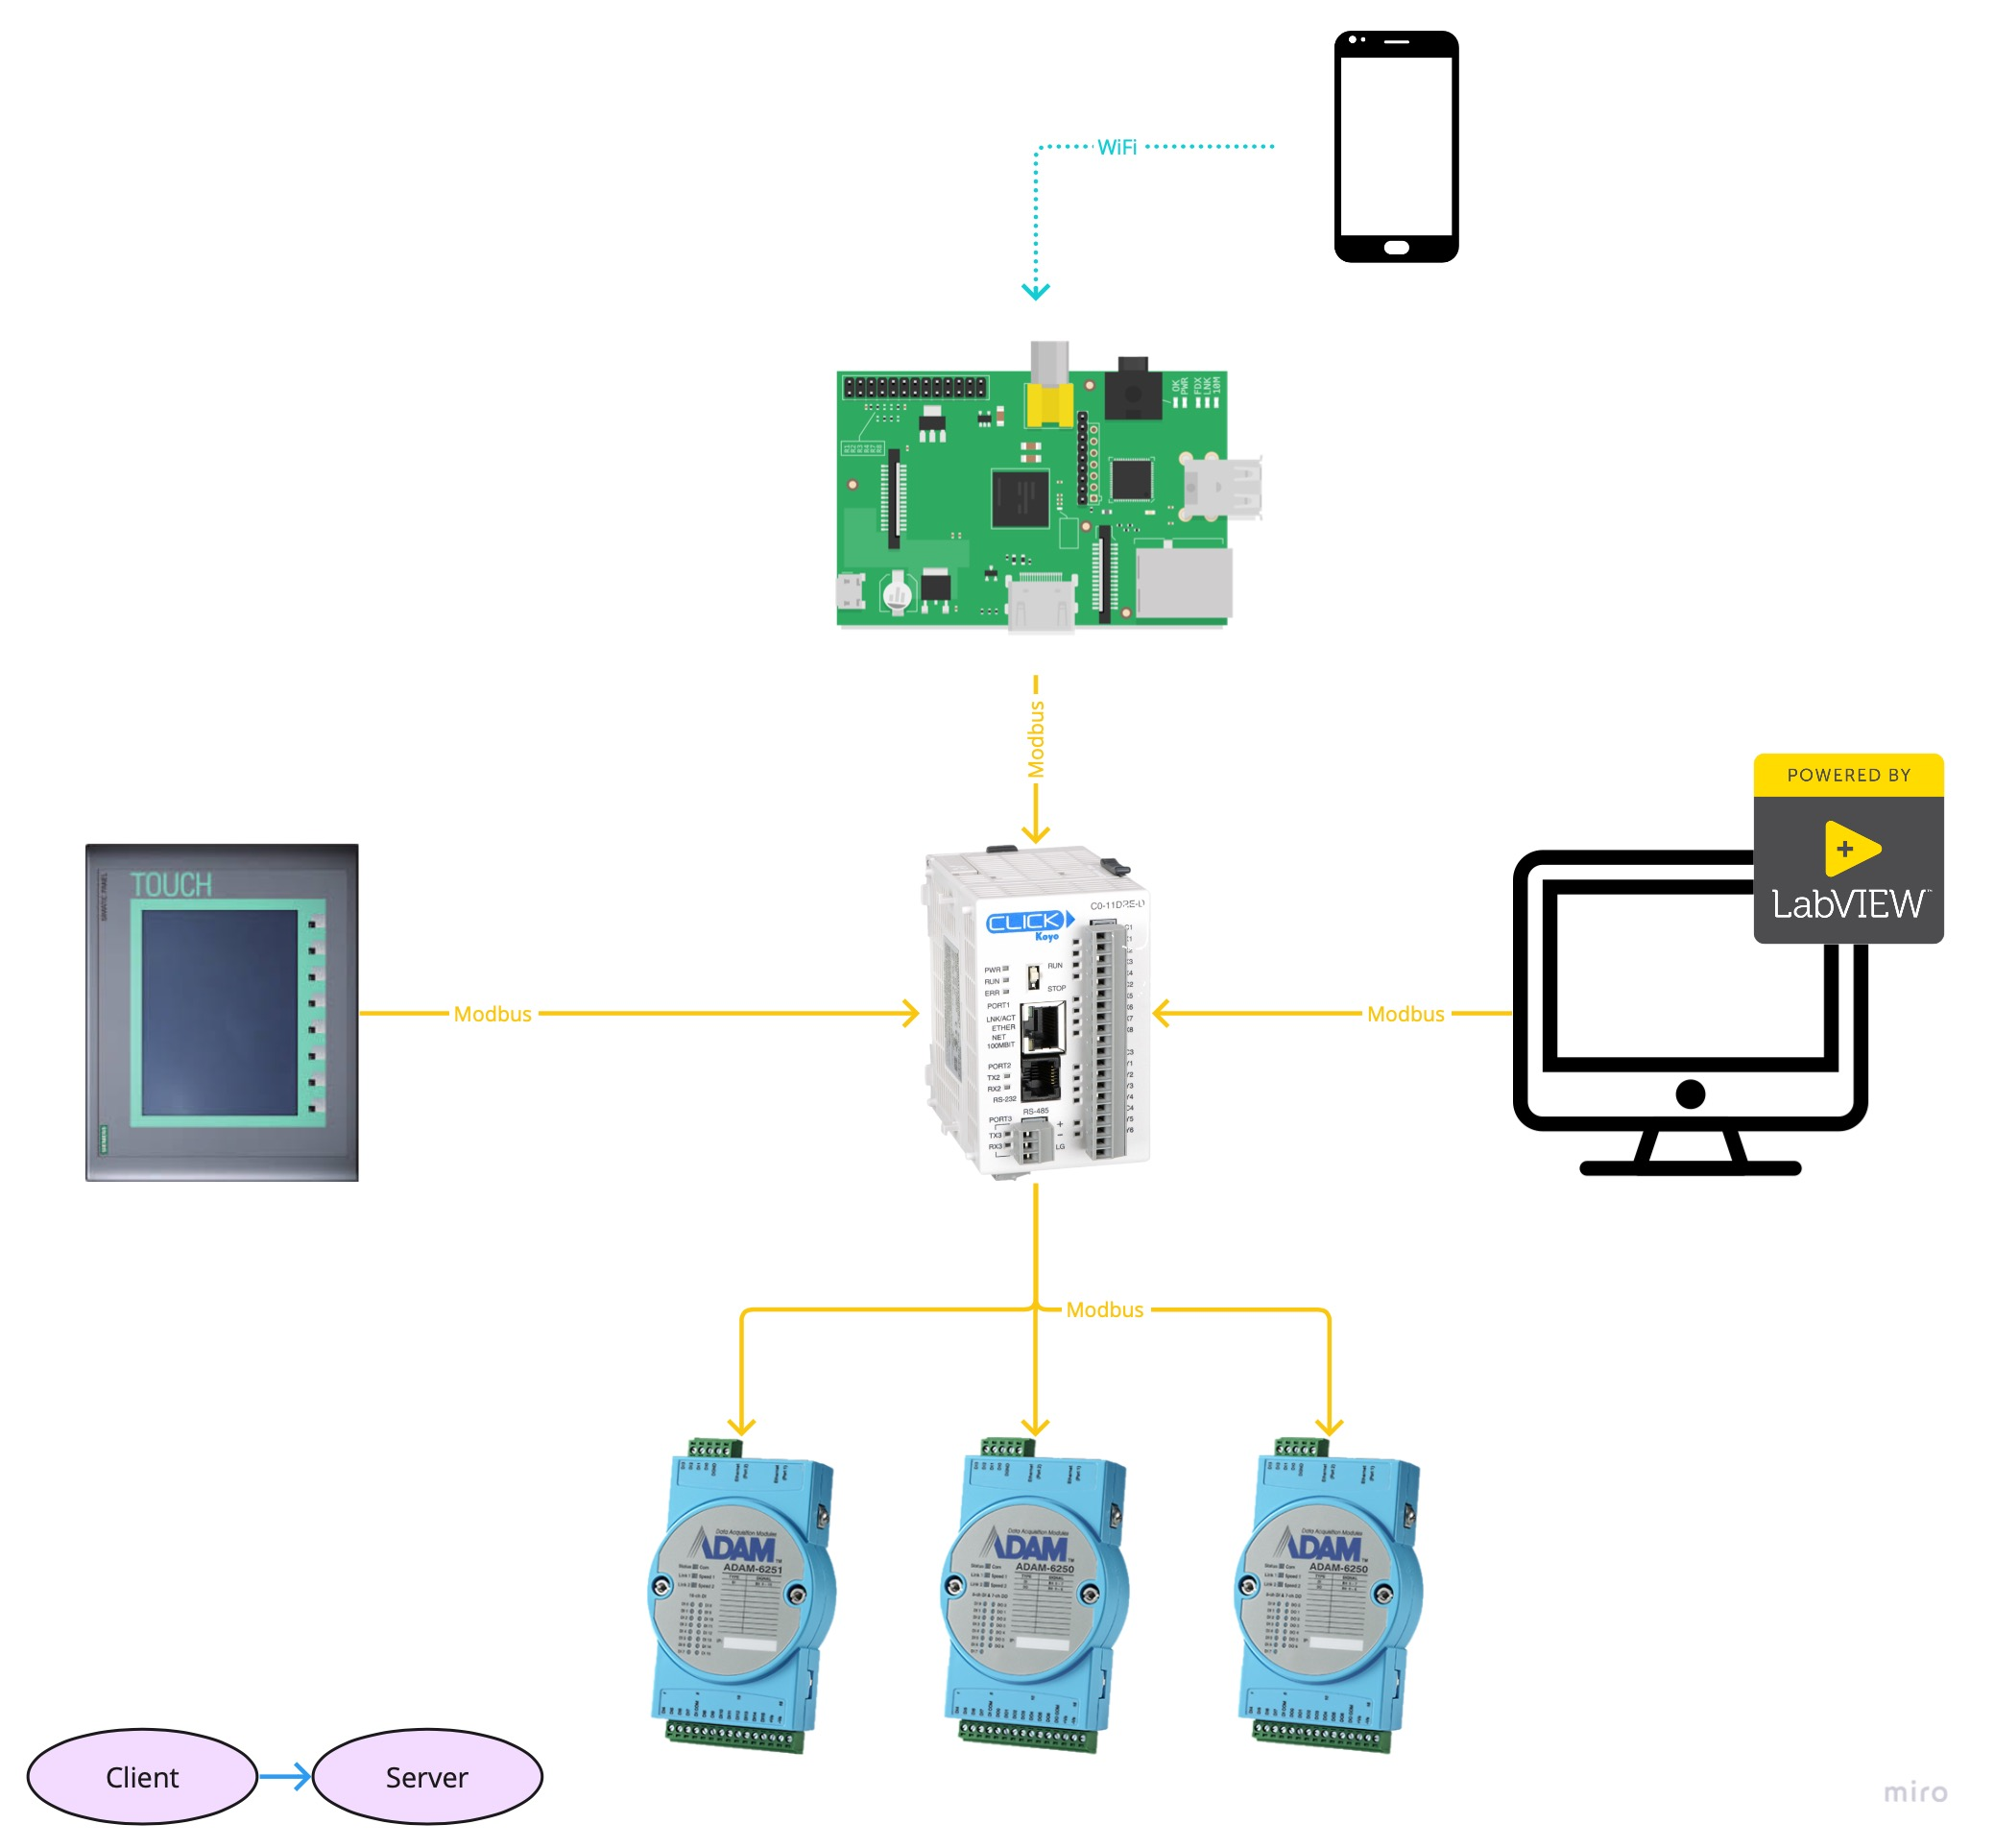
\includegraphics[width = 0.5\textwidth]{2_images/overView.jpg}
            \caption{Overview of the lolly machine network architecture.}
            \label{fig:overView}
        \end{figure} 